\begin{figure}[ht]
  \label{fig:InequalityPFGICFHWCRIC}
  \centerline{
    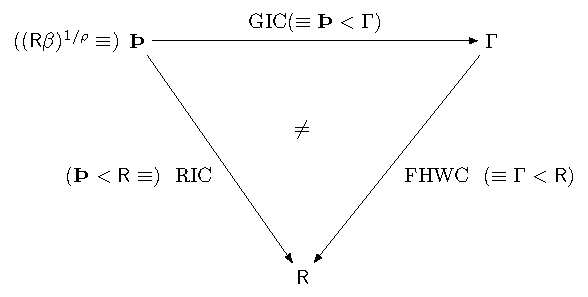
\includegraphics[width=3in]{\FigDir/InequalityPFGICFHWCRIC}
  }
  \caption{Relation of {RIC}, {GIC}, and {FHWC} in Perfect Foresight Model}
  \footnotesize{The $\neq$ signals that the arrows reflect inequality relationships.  Arrows reflect the direction of the relationship; an arrowhead points to the larger of the two quantities being compared.  For example, the topmost arrow, pointing from $\APFac$ to $\PermGroFac$, indicates that $\PermGroFac > \APFac$.}
\end{figure}
